% pdflatex presentation

\documentclass[svgnames]{beamer}
\usepackage[utf8]{inputenc}
\usepackage[T1]{fontenc}
\usepackage[sfdefault,scaled=.85,lining]{FiraSans}
\usepackage[scaled=0.85,lining]{FiraMono}
\usepackage{newtxsf}
\usepackage{rotating}
\usepackage{listings}
\usepackage{hyperref}

\usetheme{default}
\setbeamertemplate{navigation symbols}
{%
%  \hspace{3em}
%  \vbox{%
%  \hbox{\insertslidenavigationsymbol}
%  \hbox{\insertframenavigationsymbol}
%  \hbox{\insertbackfindforwardnavigationsymbol}
%  \vspace{2em}}
}

\setbeamerfont{frametitle}{family=\sffamily\firamedium}
\setbeamercolor{alerted text}{fg=red!70!black}
\setbeamercolor{structure}{fg=Navy}


\hypersetup{%
  pdftitle={Teaching programming with Jupyterhub and Nbgrader}
  ,pdfauthor={Gert-Ludwig Ingold <gert.ingold@physik.uni-augsburg.de>}
  ,pdfsubject={Talk at EuroSciPy 2018, Trento 31.8.2018}
  ,pdfkeywords={Python, Jupyterhub, nbgrader, education, EuroSciPy}
}

\definecolor{positive}{rgb}{0, 0.5, 0}
\definecolor{negative}{rgb}{0.7, 0, 0}
\definecolor{myred}{rgb}{0.8, 0, 0}
\definecolor{mygreen}{rgb}{0, 0.6, 0}
\definecolor{myblue}{rgb}{0, 0, 0.8}

\graphicspath{{./images/}}

\begin{document}

\begin{frame}[t]
 \vspace{1.5truecm}
 \begin{center}
  \structure{\huge\textbf{Teaching programming with}}\\[0.2truecm]
  \structure{\huge\textbf{Jupyterhub and Nbgrader}}\\[0.8truecm]
  \structure{\Large Gert-Ludwig Ingold}\\[0.1truecm]
  \structure{\large Universität Augsburg}
 \end{center}
\end{frame}

\begin{frame}{About me}
 \begin{itemize}
  \item theoretical physicist at the Universität Augsburg
  \item teaching programming to physicists and materials scientists since 2010
  \item involved in two Erasmus+ projects on education and computing
	\begin{itemize}
         \item iCSE4school (2015--2017)
	 \item Juypter@edu (2017--2019)
	\end{itemize}
 \end{itemize}

 \vspace{0.8truecm}
 \structure{Jupyter@edu}\qquad \raisebox{-0.2truecm}{
\includegraphics[width=0.25\textwidth]{EU_flag-Erasmus__vect_POS}}

 \begin{itemize}
  \item University of Silesia, Poland (Leader)
  \item Universität Augsburg, Germany
  \item Universidade Portucalense Infante D. Henrique, Portugal
  \item European University Cyprus, Cyprus
 \end{itemize}
\end{frame}

\begin{frame}{Grading}
 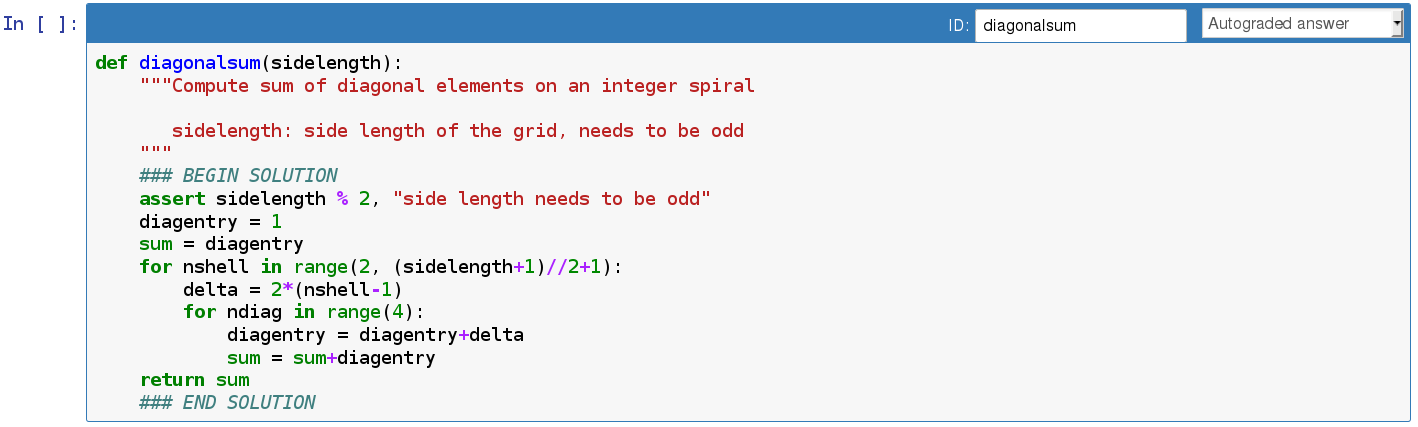
\includegraphics[width=\textwidth]{function}

 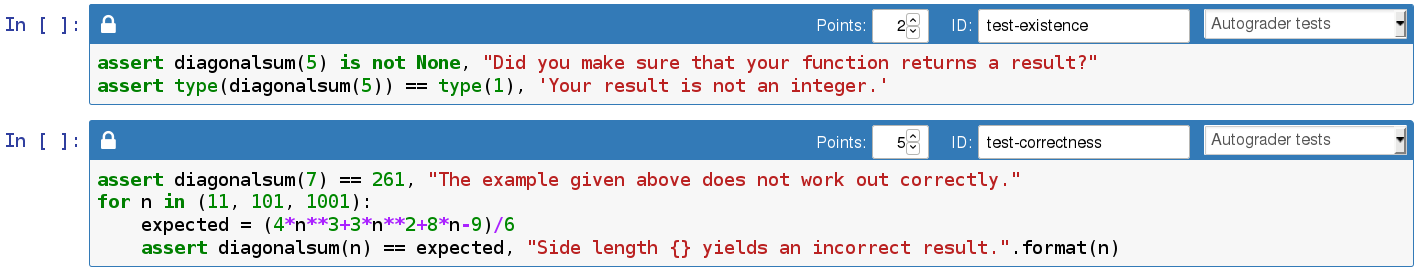
\includegraphics[width=\textwidth]{tests}
\end{frame}

\begin{frame}{Functions}
 the students' code needs to be structured in functions to be tested
 \begin{itemize}
  \item concept of a function needs to be introduced very early in the course\\
	but we will always have well defined inputs and outputs\\
	the more special aspects of a function (no argument, default arguments,
	keyword arguments, \dots) are not required
  \item students get used to logically structured code from the very beginning\\
	but they do not go through the routine of structuring the code by themselves
  \item docstrings are required to define what the function is supposed to do\\
	students get used early to the idea that a function contains a docstring\\
	but they are not writing the docstring by themselves
 \end{itemize}
\end{frame}

\begin{frame}{Grading with tests}
 \begin{itemize}
  \item Test-driven development\\
	but: tests are not developed by the students
  \item Tests allow to give feedback through error messages\\
	but: students tend to rely on this feedback instead of developing their own critical view on their code\\
	potential problem of incomplete tests
  \item ``Stupid mistakes'' will be made even when students get more advanced\\
	also test for the simple things: are results returned, do they have the correct type, \dots\\
	``trivial'' standard tests + tests of specific functionality
  \item The test should not disclose the solution.
 \end{itemize}
\end{frame}

\begin{frame}{Coping with heterogeneity}
 \begin{itemize}
  \item students without programming experience and (sometimes) code writing apprehension
  \item students with knowledge in another programming language\\
	code often does not look very pythonic, example: loop over objects vs. loop over indices
 \end{itemize}

 students with programming experience should not be bored and should obtain an interesting result from their code

 \begin{itemize}
  \item scientific applications are often considered as an extra mental burden
 \end{itemize}
\end{frame}

\begin{frame}{Examples of exercises}

 \vspace{-0.7truecm}
 \begin{columns}[t]
  \begin{column}{0.5\textwidth}
   \begin{center}
    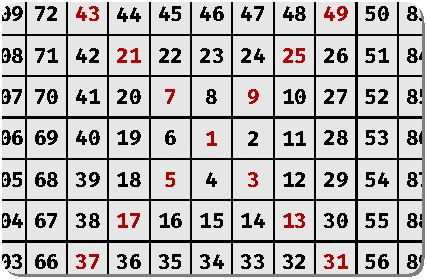
\includegraphics[width=0.8\textwidth]{spiral}

    selected problems from\\[-0.05truecm] Project Euler (\url{projecteuler.net})
   \end{center}
  \end{column}%
  \begin{column}{0.5\textwidth}
   \begin{center}
    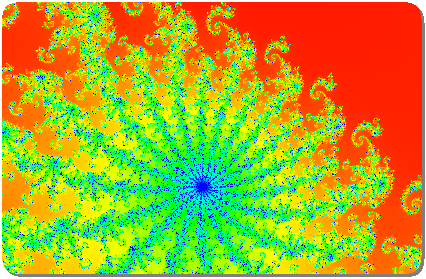
\includegraphics[width=0.8\textwidth]{julia}

    Julia set
   \end{center}
  \end{column}%
 \end{columns}

 \begin{columns}[t]
  \begin{column}{0.5\textwidth}
   \begin{center}
    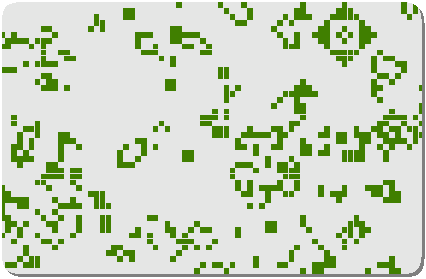
\includegraphics[width=0.8\textwidth]{conway}

    Conway's game of life
   \end{center}
  \end{column}%
  \begin{column}{0.5\textwidth}
   \begin{center}
    
\includegraphics[width=0.8\textwidth]{pi}

    $\pi$ to a few thousand digits
   \end{center}
  \end{column}%
 \end{columns}

 \vspace{0.4truecm}
 {\scriptsize\url{https://github.com/marcinofulus/jupyter4edu/tree/master/augsburg/exercises}}
\end{frame}

\begin{frame}{Branching paths}
 \only<1>{%
  \begin{columns}
   \begin{column}{0.3\textwidth}
    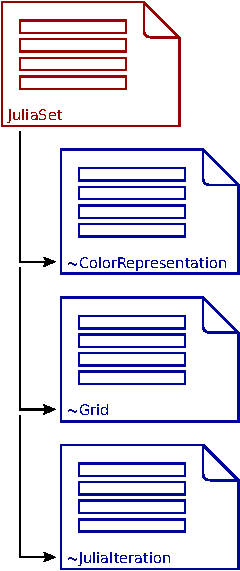
\includegraphics[height=0.8\textheight]{branching_1}
   \end{column}%
   \begin{column}{0.7\textwidth}
    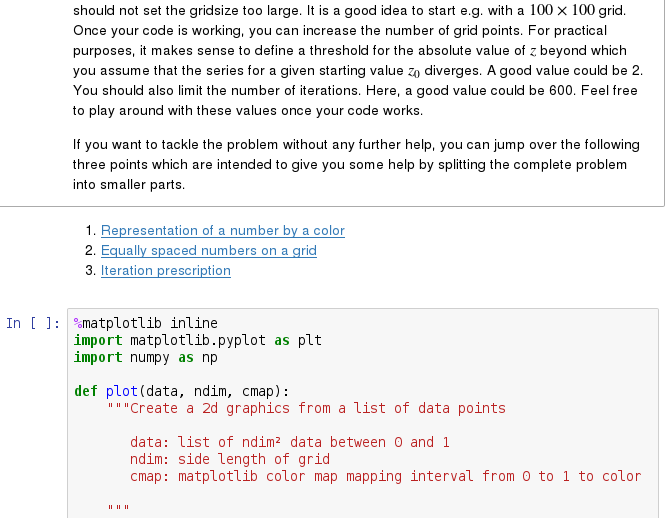
\includegraphics[width=\textwidth]{JuliaSet_screenshot}
   \end{column}
  \end{columns}
 }%
 \only<2>{%
  \begin{columns}
   \begin{column}{0.3\textwidth}
    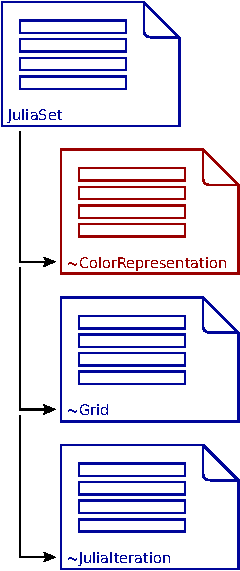
\includegraphics[height=0.8\textheight]{branching_2}
   \end{column}%
   \begin{column}{0.7\textwidth}
    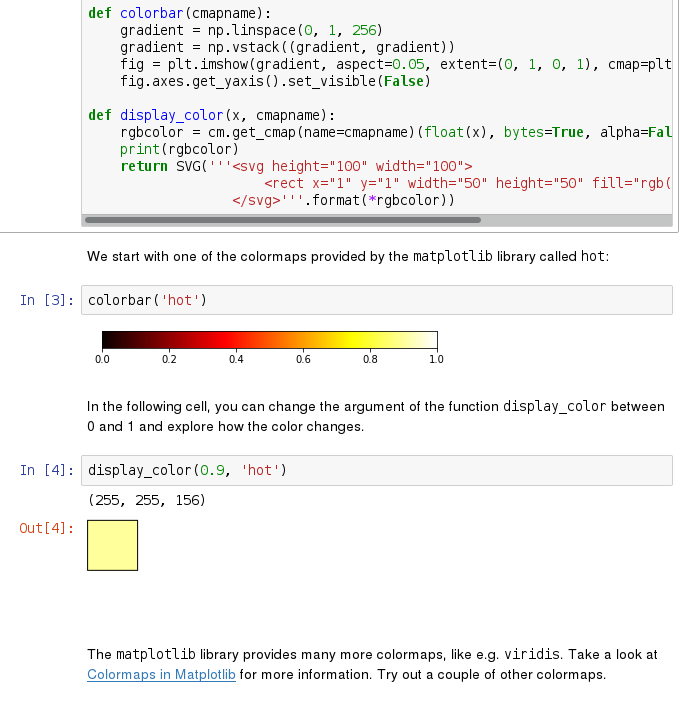
\includegraphics[width=\textwidth]{ColorRepresentation_screenshot}
   \end{column}
  \end{columns}
 }%
 \only<3>{%
  \begin{columns}
   \begin{column}{0.3\textwidth}
    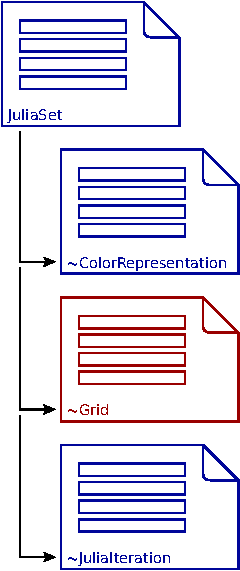
\includegraphics[height=0.8\textheight]{branching_3}
   \end{column}%
   \begin{column}{0.7\textwidth}
    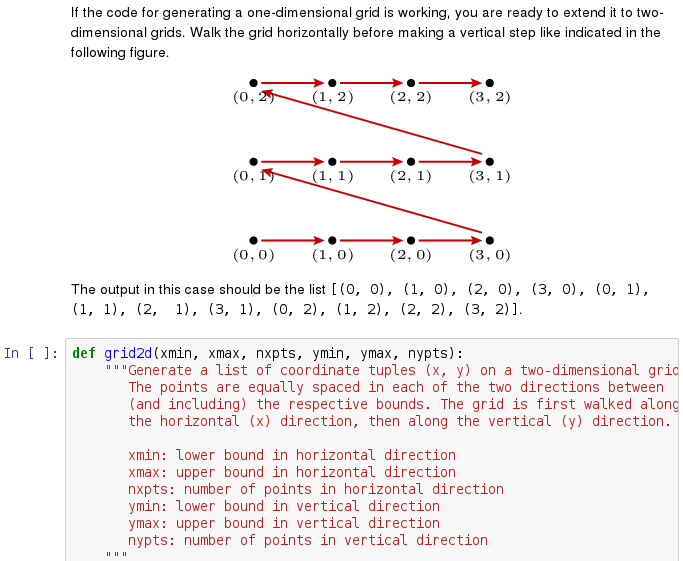
\includegraphics[width=\textwidth]{Grid_screenshot}
   \end{column}
  \end{columns}
 }%
 \only<4>{%
  \begin{columns}
   \begin{column}{0.3\textwidth}
    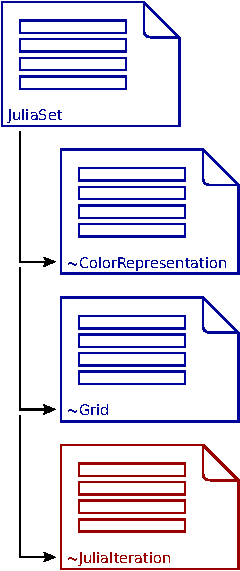
\includegraphics[height=0.8\textheight]{branching_4}
   \end{column}%
   \begin{column}{0.7\textwidth}
    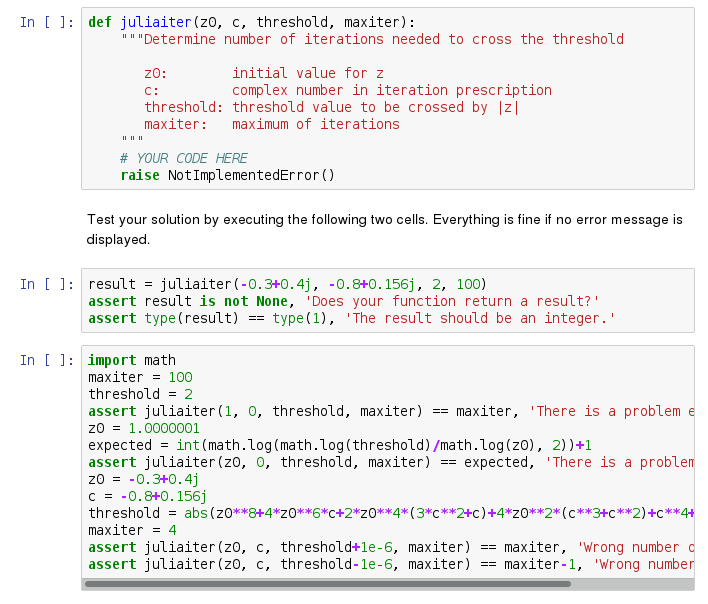
\includegraphics[width=\textwidth]{JuliaIteration_screenshot}
   \end{column}
  \end{columns}
 }
\end{frame}

\begin{frame}{Branching paths}
 \begin{itemize}
  \item individual path through problem possible
  \item other notebooks are opened in new tabs, it is easy to lose track
 \end{itemize}
\end{frame}

\end{document}
